\documentclass[a4paper,10pt]{article}
\usepackage[top=2.5cm,bottom=2.5cm,left=2.5cm,right=2.5cm,showframe]{geometry}
\usepackage{xcolor,fancyhdr}
\usepackage{tikz}
\usepackage{amsmath,amssymb,amsthm,amsfonts}
\usepackage{stmaryrd}

\usepackage{lineno}
\linenumbers
\setpagewiselinenumbers

%%%%%%%%%%%%%  PLEASE DO NOT EDIT ANY OF THE LINES ABOVE %%%%%%%%%%%%%%%
% Insert your text between "\begin{document}" and "\end{document}" below. 
% The total length of your summary notes should not exceed 2 sides of a
% single sheet of A4, with maximum 58 lines of text per page.
%%%%%%%%%%%%%%%%%%%%%%%%%%%%%%%%%%%%%%%%%%%%%%%%%%%%%%%%%%%%%%%%%%%%%%%%

\newcommand{\x}{\mathbf{x}}
\newcommand{\uvec}{\mathbf{u}}
\newcommand{\vvec}{\mathbf{v}}
\newcommand{\w}{\mathbf{w}}
\usepackage{graphicx}
\graphicspath{ { ./NS/ } } 
\usepackage{caption}
\usepackage{subcaption}

\begin{document}
\include{stylefile}


\textbf{\S1 Linear System}
$\dot \x = A\x$ \hspace{0.5cm} $\x(0) = \x_0 \Longrightarrow \x(t) = e^{tA}\x_0$

(If $A=BCB^{-1}$, $e^{tA} = Be^{tC}B^{-1} = B \text{diag} (e^{\lambda_1 t},\cdots,\lambda_n t)B^{-1}$)

\underline{2D} $\lambda_1 \lambda_2 < 0$ Saddle \hspace{0.3cm} $\lambda_1 \lambda_2 > 0$ Node \hspace{0.3cm} 

$\lambda_1 = \lambda_2$ and $\dim E_\lambda = 1$ Degenerate node ($y1 = y_{10}e^{\lambda t} + y_{20}te^{\lambda t}$, $y_2 = y_{20}e^{\lambda t}$): Secular, but stability still determined by sign.

$\lambda_1 = a+ib$, $\lambda_2 = a-ib$ $\Longrightarrow$ $a=0$ Center \hspace{0.5cm} $a \neq 0$ Focus (Spiral)

Hyperbolic System: All eigval $\neq 0$ \hspace{2cm}

Eigenspace is invariant.

\underline{Lin Subsp}: For $A\w_j = \lambda_j \w_j$, $\w_j = \uvec_j + i\vvec_j$, $\lambda_j = a_j + ib_j$ (For nonsemisimple, $(A-\lambda I)^k \w = 0$)

$E^s = \text{Span}(\uvec_j, \vvec_j | a_j < 0)$ \hspace{0.5cm} $E^c = \text{Span}(\uvec_j, \vvec_j | a_j = 0)$ \hspace{0.5cm} $E^u = \text{Span}(\uvec_j, \vvec_j | a_j > 0)$

\rule{6cm}{0.4pt}

\textbf{\S2 Nonlinear Systems}

\underline{Orbit} of $\x_0$: curve $\Gamma_{\x_0} \subset E$: $\Gamma_{\x_0} = \left\{ \x(t;\x_0) | t\in\mathbb{R} \right\}$

\underline{Flow} is the map $\varphi_t:E\rightarrow E$ s.t. $\varphi_t(\x_0) = \x(t;\x_0)$

$\mathbf{p} \in E$ is \underline{$\omega$-limit pt} of $\varphi_t(\x)$: $\exists t_1 < t_2< \cdots < t_n \rightarrow \infty$ s.t. $\lim_{i\rightarrow \infty}\phi_{t_i} = \mathbf{p}$ \hspace{0.5cm} cf) $\alpha$-lim pt

Closed invariant set $A$ \underline{Attracting set} if $\exists$ neighborhood $U$ of $A$ s.t. $\varphi_t(U) \subset U$ and $A = \cap_{t>0} \varphi_t(U)$

\underline{Domain of attraction} $D(A) = \cup_{t\leq 0}\varphi_t(U)$ (AKA set of all IC s.t. have A as $\omega$-lim set)

\underline{Attractor}: Attracting set with a dense orbit.

\underline{Poincar\'{e}-Bendixson Thrm}: $E\subset \mathbb{R}^2$ open, $\mathbf{f} \in C^1 (E)$. If $D \subset E$ compact (closed bdd) s.t. $\x(t) \in D$ for all $t \geq 0$ where $\dot \x = \mathbf{f} (\x)$, then orbit is either a limit cycle or approaches a limit cycle, or approaches an equilibrium.

Fixed point $\x_0$ \underline{Lyapunov stable}: $\forall \epsilon > 0 \exists \delta > 0$ s.t. $\forall \x \in B_\delta (\x_0)$ and $t \geq 0$, $\varphi_t(\x) \in B_\epsilon (\x_0)$

Fixed point $\x_0$ \underline{asympt. stable}: (i) Lyapunov and (ii) $\exists \delta > 0$ s.t. $\varphi_t(\x) \rightarrow \x_0$ as $t\rightarrow \infty$ $\forall x\in B_\delta (\x_0)$

\rule{6cm}{0.4pt}

\textbf{Lyapunov Function} $V(\x_0) = 0, V(\x) > 0 \forall \x \in W \setminus \left\{ \x_0 \right\}$ \hspace{0.5cm} Tip: $\dot V(\x)=\nabla V(\x) \cdot \dot \x = \nabla V(\x) \cdot {\mathbf{f}} (\x)$

(i) $\dot V(\x) \leq 0$ $\forall \x \in W \setminus \left\{ \x_0 \right\} \Longrightarrow$ Stable

(ii) $\dot V(\x) < 0$ $\forall \x \in W \setminus \left\{ \x_0 \right\} \Longrightarrow$ Asymptotic Stable

(iii) $\dot V(\x) > 0$ $\forall \x \in W \setminus \left\{ \x_0 \right\} \Longrightarrow$ Unstable

\rule{6cm}{0.4pt}

\textbf{\S3 Local Analysis}

From linearized system around origin,

$W^s(0) = \left\{ (x,y) \in \mathbb{R}^2 | \varphi_t (x,y) \rightarrow 0 \text{ as } t \rightarrow \infty \right\}$ , $W^u(0) = \left\{ (x,y) \in \mathbb{R}^2 | \varphi_t (x,y) \rightarrow 0 \text{ as } t \rightarrow -\infty \right\}$

\underline{Center manifold}: (i) Tangent to $E^c$ at $\x_0$ (ii) of class $C^r$ (where $f\in C^R(E)$) (iii) invar under flow.
(Interested in smoothest center manifold)

\underline{Shadowing Theorem}: $\left( \x_0, \mathbf{y}_0 \right)$ close enough to origin, $(\x(t),\mathbf{y}(t))$ solution $\Longrightarrow \exists \tilde \x(t)$ on center man. s.t. 
$
\begin{cases}
	\x(t) = \tilde \x(t) + O(e^{-\gamma t}) \\
	\mathbf{y}(t) = \mathbf{h}\left( \tilde \x(t) \right) + O(e^{-\gamma t})
\end{cases}
$
for some const $\gamma > 0$.

\rule{6cm}{0.4pt}

\textbf{\S4. Bifurcations}

\underline{Topological equivalence} Two vector field $\mathbf{f}$ and $\mathbf{g}$ and resp. flows $\varphi_t (\x)$ and $\psi_t (\x)$ are top.equi. if $\exists$ homeomorphism (1-1,cts,cts inv) $\mathbf{h}:\mathbb{R}^n \rightarrow \mathbb{R}^n$ and $\tau(t,\x) \rightarrow \mathbb{R}$ strict. inc. on $t$ s.t. $\tau(t+s,\x) = \tau(s,\x) + \tau(t,\varphi_s(\x))$

\underline{Structural Stability}: VF $\mathbf{f}$ structurally stable if $\forall$ ctsly diff. VF $\mathbf{v}$, $\exists \epsilon_v > 0$ s.t. $\mathbf{f}$ is top.equiv to $\mathbf{f} + \epsilon \mathbf{v} \forall 0 < \epsilon < \epsilon_v$

\underline{Bifurcation Pt}: $\mathbf{\mu}_c$ point in param. space where $f$ is not structurally stable.

\underline{Bifurcation}: Change in structure of the solution.

Step-by-Step: Find fixed point. Compute Jacobian (w.r.t $\mu$ as a const) around a fixed pt and set it to zero. Check Hopf.

Examples
(i) $\dot x = \mu x - x^2$ (Transcritical, fp:$x=0,\mu$) (ii) $\dot x = \mu -x^2$ (Saddle, fp:$x=\pm \mu^{1/2}$)

(iii) $\dot x = \mu x - x^3$ (Sup.crit pitch, fp:$x=0,\pm \mu^{1/2}$) (iv) $\dot x = -\mu x + x^3$ (Sub.crit pitch, fp:$x=0,\pm \mu^{1/2}$)

% IMAGE
\begin{figure}[h]
	\centering
	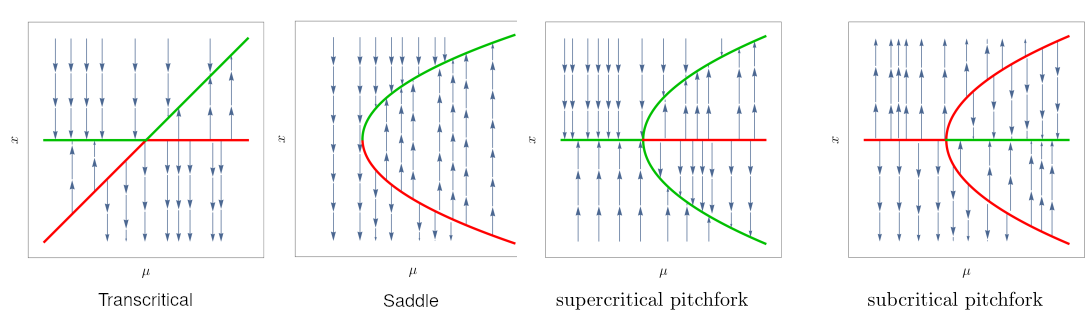
\includegraphics[scale=2.2]{Bifeg.png}
\end{figure}

\rule{6cm}{0.4pt}

\textbf{\S5 Local Analysis of Maps} $\x_{n+1} = \mathbf{G}(\x_n)$

$E^s = \text{Span} (\uvec_j, \vvec_j | |\lambda_j| < 1)$ \hspace{0.5cm}
$E^c = \text{Span} (\uvec_j, \vvec_j | |\lambda_j| = 1)$ \hspace{0.5cm}
$E^u = \text{Span} (\uvec_j, \vvec_j | |\lambda_j| > 1)$

\underline{Stability}: Fixed pt $\x_0$ s.t. $\forall \epsilon > 0$, $\exists \delta > 0$ s.t. $\forall \x \in B_\delta(\x_0)$ for all $n\in\mathbb{Z}^+$

\underline{Asympt Stability}: $\x_0$ s.t. stable and $\exists \delta > 0$ s.t. $\forall \x \in B_\delta (\x_0)$, $\mathbf{G}^{(n)}(\x) \rightarrow \x_0$ as $n \rightarrow \infty$

$\forall \x \in W_{loc}^s$, $\mathbf{G}^{(n)}\rightarrow \x_0$ as $n \rightarrow \infty$ \hspace{0.5cm}
$\forall \x \in W_{loc}^u$, $\mathbf{G}^{(n)}\rightarrow \x_0$ as $n \rightarrow -\infty$ 

Periodic orbit $\Gamma$ is \underline{Lyapunov stable} if $\forall \epsilon > 0$: $\exists \delta > 0$ s.t. $\varphi_t(\x) \in U_\epsilon(\Gamma)$ for all $t \geq 0$ and $\x \in U_\delta$

Periodic orbit $\Gamma$ \underline{Asympt stable} if Lyapunov + $\exists \delta > 0$ s.t. $d(\varphi_t(\x), \Gamma)$ as $t\rightarrow\infty$ for all $\x \in U_\delta$

Poincar\'{e} Map Traversality: $\mathbf{n} \cdot \mathbf{f}(\x_0) > 0$

\rule{6cm}{0.4pt}

\textbf{\S6 Limit Cycles and Hopf Bifur}

\underline{Poincar\'{e}-Lindstedt Method}: $\ddot x + x = \epsilon f(x)$

Define timescale $\tau = \omega t$ s.t. $x(\tau + 2\pi, \epsilon) = x(\tau,\epsilon)$ \hspace{0.5cm} (Tip: $\frac{d}{dt} = \omega \frac{d}{d\tau}$)

Translation of time: $\dot{x} = 0$ at $t=0$ \hspace{0.5cm} Amplitude of oscillation: $a = x(0,\epsilon)$

Expansion: $\omega = \omega_0 + \epsilon \omega_1 + \epsilon^2 \omega_2 + \cdots$ \hspace{0.5cm} $x(\tau,\epsilon) = x_0(\tau) + \epsilon x_1 (\tau) + \epsilon^2 x_2 (\tau)$ (No secular solution)

(Tip: $\cos^2 \tau = \frac{1+\cos 2\tau}{2}$,$\cos^3 \tau = \frac{3 \cos \tau + \cos 3\tau}{4}$ )

\rule{6cm}{0.4pt}

\textbf{Hopf} $\Re (\lambda) = 0$ at $\mu = \mu_c$ \hspace{0.3cm}
$\dot r = d\mu r + ar^3$ \hspace{0.3cm}
$\dot \theta = \omega + c\mu + br^2$ \hspace{0.3cm}
$d = {\frac{d}{d\mu}\Re{\lambda (\mu)} |} _{\mu = \mu_c}$, 
$c = {\frac{d}{d\mu}\Im{\lambda (\mu)} |}_{\mu = \mu_c}$

$\dot x = \mu x -\omega y +f(x,y)$ \hspace{0.5cm}
$\dot y = \omega y + \mu y + g(x,y)$

$\Longrightarrow a=\frac{1}{16\omega}\left( \left( f_{xxx} + f_{xyy} + g_{xxy} + g_{yyy} \right)\omega + f_{xy}\left( f_{xx} + f_{yy} \right) - g_{xy}\left( g_{xx} + g_{yy} \right) - f_{xx}g_{xx} + f_{yy}g_{yy} \right)$

\rule{6cm}{0.4pt}

\textbf{Local Bifur}

\underline{$\lambda = 1$}: eg) $x + \mu -x^2$ saddle \hspace{0.5cm} $x + \mu x -x^2$ transcritical \hspace{0.5cm} $x + \mu x -x^3$ pitchfork

\underline{Bifur of Periodic Orbit}: Seek Poincar\'{e} map s.t. $\delta \rightarrow \delta + \frac{\delta^2}{2}P_rr(1,0) + \mu P_\mu (1,0)$. For $\dot r = f(r,\theta,\mu)$, $P_\mu(1,0) = \int_0^{2\pi} f_\mu(1,\theta,0) dt$, $P_r(1,0) = 1$, $P_{rr}(1,0) = \int_0^{2\pi} f_{rr}(1,\theta,0) dt$ 

\underline{$\lambda = -1$}: eg) $f(x,\mu) = -x -\mu x + x^3$ Period-doubling

\rule{6cm}{0.4pt}

\textbf{\S7 Global Bifur, Homoclinic Chaos, Melnikov's Method} $\dot \x = \mathbf{f}(\x) + \epsilon \mathbf{g}(\x, t)$

$f$ has \underline{sensitivity to IC} on $\Lambda$ if $\exists \epsilon > 0$ s.t. for any $p \in \Lambda$ and any neighborhood $U$ of $p$, $\exists p' \in U$ and $n\in\mathbb{N}$ s.t. $|f^n(p) - f^n(p')| > \epsilon$

$f$ \underline{topolo. transitive} on $\Lambda$ if for any open $U$,$V \subset \Lambda$, $\exists n \in \mathbb{Z}$ s.t. $f^n (U) \cap V \neq \emptyset$

$\Lambda$ invar compact set for invertible $f$. $f$ \underline{chaotic} on $\Lambda$ if $\exists$ sensitivity to IC on $\Lambda$ and topo. transitive on $\Lambda$

Assumption: $\mathbf{f}(\x) = (f_1,f_2) = \left( \frac{\partial H}{\partial y}, -\frac{\partial H}{\partial x} \right)$ (Hamiltonian)

\underline{Melnikov Function}: $M(t_0) = \int_{\infty}^{\infty} \mathbf{f}(\mathbf{q}_0 (t-t_0)) \wedge \mathbf{g}(\mathbf{q}_0 (t-t_0),t) dt$ ($\x = \mathbf{q}_0(t)$ for $\epsilon = 0$, homoclinic)

$M$ has a simple zero at a point $t_0 = \tau$, then $P_\epsilon$ has a transverse homoclinic point for sufficiently small $\epsilon > 0$ \hspace{0.5cm}

If $M(t_0) > 0$ or $M(t_0) < 0$ for all $t_0$, then $W^s(\x_\epsilon) \cap W^u (\x_\epsilon) = \emptyset$

Eg) Duffing Oscil. $\ddot x = x - x^3 - \delta \dot x + \gamma \cos{t}$

$\dot x = y = \pm x {\left( 1 - \frac{x^{2}}{2} \right)}^{\frac{1}{2}} \Longrightarrow
(x_0(t),y_0(t)) = \mathbf{q}_0(t) = \pm (\sqrt{2} \text{sech }{t}, -\sqrt{2} \text{sech }{t} \tanh{t})
$

\end{document}
